\section{Extending the \METHOD~Structured Language}
\label{section:extendability}

\begin{figure}[t]
    \centering
    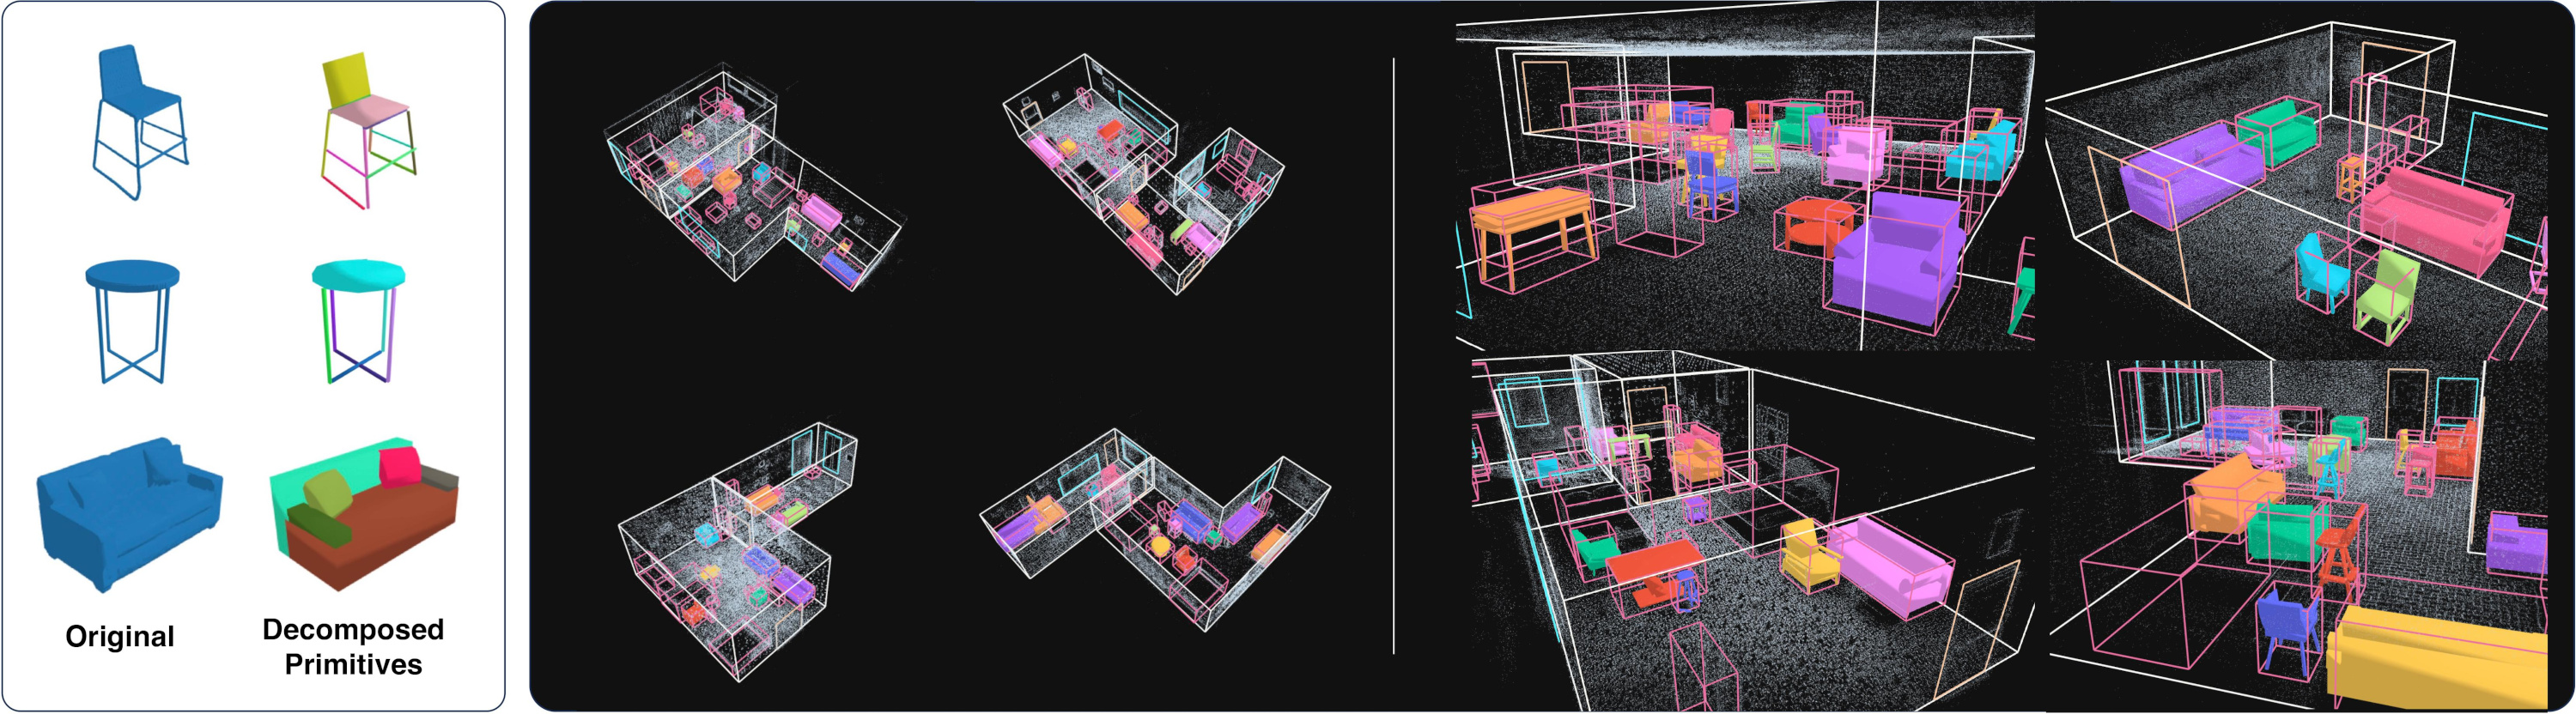
\includegraphics[width=\textwidth]{figs/ase_primitives.jpg}
    \caption{Example scene reconstructions on scenes from \DatasetName{}.
        (left) Visualisation of the decomposed meshes used to create \texttt{make\_prim} training pairs.
        (right) Views of full scene predictions, as well as close ups highlighting the fidelity of object reconstruction through the prediction volumetric primitives enabled by \texttt{make\_prim}.}
    \label{fig:commandVisExamples1}
\end{figure}



A key advantage offered by \METHOD's structured language prediction paradigm is that the expressiveness of its reconstruction can be tailored without requiring a change to the method. Up to now, we have focussed on showcasing the efficacy of \METHOD~for representing simple layout elements and objects as bounding boxes. In this section, we showcase this characteristic by increasing the fidelity of our scene representation by introducing coarse 3D object reconstruction. 



\subsection{Objects as Volumetric Primitives}
We turn to a language based on volumetric primitives, motivated by works such as~\cite{tulsiani2017learning,yang2021unsupervised}. 
Using simple primitives such as cuboids and extruded cylinders, enables us to coarsely represent arbitrary object categories while maintaining object semantics (e.g. tabletops can be represented by a single cuboid). 
Thus, this language can describe many object categories simultaneously.

This representation requires only one additional command over the layout and box commands already discussed previously, namely:
\begin{lstlisting}[language=StructuredLanguage]
make_prim: bbox_id, prim_num, class, center_x, center_y, center_z, angle_x, angle_y, angle_z, scale_x, scale_y, scale_z
\end{lstlisting}
This command and its parameters describe a volumetric primitive (cuboid or extruded cylinder) via its 3D center, 3D rotation, and 3D scale. The \texttt{prim\_num} parameter can be associated with semantics, e.g. tabletops of different tables typically have the same \texttt{prim\_num}.

\begin{figure*}[t]
    \centering
    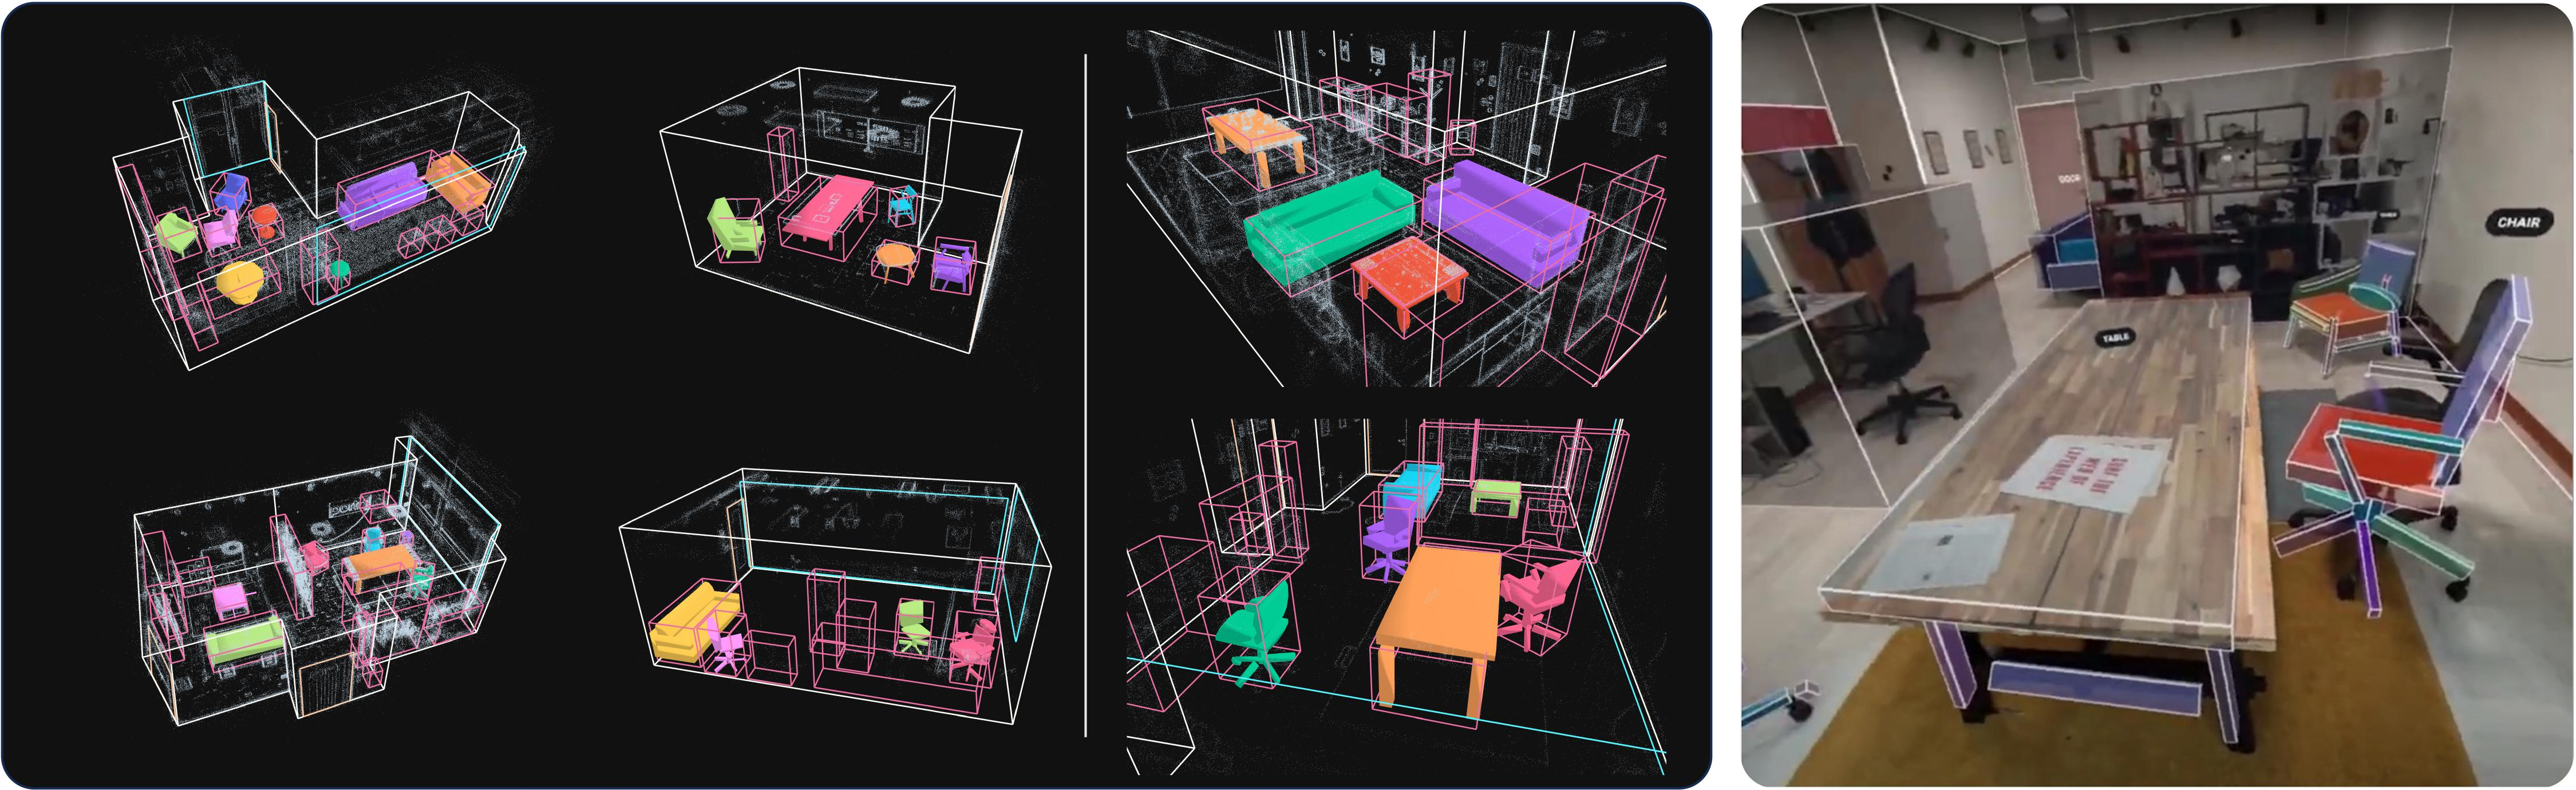
\includegraphics[width=\textwidth]{figs/real_scenes.jpg}
    \caption{Example scene reconstructions on \textbf{real scenes} with the addition of the \texttt{make\_prim} command. Note that \METHOD{} was trained only on synthetic data.}
    \label{fig:extensions}
\end{figure*}

\subsubsection{Dataset.}
To obtain ground truth \texttt{make\_prim} commands that align with the objects in \DatasetName, we first run an extension of Yang~\etal~\cite{yang2021unsupervised} to obtain cuboid and extruded cylinder primitives of a database of 3D CAD models (ABO~\cite{collins2022abo}, which was used to populate \DatasetName). See Figure~\ref{fig:commandVisExamples1} (left) for example decompositions. For this proof-of-concept experiment, we use three categories: \textit{table}, \textit{chair}, and \textit{sofa}. We then convert these decomposed primitives into \texttt{make\_prim} commands that are aligned with the objects in the dataset, which results in training pairs. 


\subsubsection{Results.} 
We show qualitative results on \DatasetName{} in Figure~\ref{fig:commandVisExamples1}.
In Figure~\ref{fig:extensions},
we show inferences in a few real-world environments
despite only having trained on our simulated dataset.
These results demonstrate that \METHOD{}'s general purpose architecture is capable of coarsely reconstructing objects of multiple categories through addition of a new command.
% Importantly, recall that the joint inference of both layout elements and coarse object reconstruction are done with a single general purpose architecture.




\subsection{Further Extensions}
In this section, we have explored just one extension of \METHOD's structured scene language in order to demonstrate its flexibility. The result was greatly increased expressiveness of the scene reconstruction. 
In Appendix~\ref{app:extensions},
% In the supplement, 
we include additional explorations that can further increase the fidelity and accuracy of \METHOD's reconstructions. These explorations include reconstructing curved walls, inferring object states (such as door opening angles), as well as direct prediction of parametric models using object models deployed commonly by tech artists (e.g., blender geometry nodes) for object reconstruction.
